% Options for packages loaded elsewhere
\PassOptionsToPackage{unicode}{hyperref}
\PassOptionsToPackage{hyphens}{url}
%
\documentclass[
]{article}
\usepackage{amsmath,amssymb}
\usepackage{lmodern}
\usepackage{iftex}
\ifPDFTeX
  \usepackage[T1]{fontenc}
  \usepackage[utf8]{inputenc}
  \usepackage{textcomp} % provide euro and other symbols
\else % if luatex or xetex
  \usepackage{unicode-math}
  \defaultfontfeatures{Scale=MatchLowercase}
  \defaultfontfeatures[\rmfamily]{Ligatures=TeX,Scale=1}
\fi
% Use upquote if available, for straight quotes in verbatim environments
\IfFileExists{upquote.sty}{\usepackage{upquote}}{}
\IfFileExists{microtype.sty}{% use microtype if available
  \usepackage[]{microtype}
  \UseMicrotypeSet[protrusion]{basicmath} % disable protrusion for tt fonts
}{}
\makeatletter
\@ifundefined{KOMAClassName}{% if non-KOMA class
  \IfFileExists{parskip.sty}{%
    \usepackage{parskip}
  }{% else
    \setlength{\parindent}{0pt}
    \setlength{\parskip}{6pt plus 2pt minus 1pt}}
}{% if KOMA class
  \KOMAoptions{parskip=half}}
\makeatother
\usepackage{xcolor}
\IfFileExists{xurl.sty}{\usepackage{xurl}}{} % add URL line breaks if available
\IfFileExists{bookmark.sty}{\usepackage{bookmark}}{\usepackage{hyperref}}
\hypersetup{
  pdftitle={Social Media Intelligence Project},
  pdfauthor={Elisabeth Putri - 20306250},
  hidelinks,
  pdfcreator={LaTeX via pandoc}}
\urlstyle{same} % disable monospaced font for URLs
\usepackage[margin=1in]{geometry}
\usepackage{color}
\usepackage{fancyvrb}
\newcommand{\VerbBar}{|}
\newcommand{\VERB}{\Verb[commandchars=\\\{\}]}
\DefineVerbatimEnvironment{Highlighting}{Verbatim}{commandchars=\\\{\}}
% Add ',fontsize=\small' for more characters per line
\usepackage{framed}
\definecolor{shadecolor}{RGB}{248,248,248}
\newenvironment{Shaded}{\begin{snugshade}}{\end{snugshade}}
\newcommand{\AlertTok}[1]{\textcolor[rgb]{0.94,0.16,0.16}{#1}}
\newcommand{\AnnotationTok}[1]{\textcolor[rgb]{0.56,0.35,0.01}{\textbf{\textit{#1}}}}
\newcommand{\AttributeTok}[1]{\textcolor[rgb]{0.77,0.63,0.00}{#1}}
\newcommand{\BaseNTok}[1]{\textcolor[rgb]{0.00,0.00,0.81}{#1}}
\newcommand{\BuiltInTok}[1]{#1}
\newcommand{\CharTok}[1]{\textcolor[rgb]{0.31,0.60,0.02}{#1}}
\newcommand{\CommentTok}[1]{\textcolor[rgb]{0.56,0.35,0.01}{\textit{#1}}}
\newcommand{\CommentVarTok}[1]{\textcolor[rgb]{0.56,0.35,0.01}{\textbf{\textit{#1}}}}
\newcommand{\ConstantTok}[1]{\textcolor[rgb]{0.00,0.00,0.00}{#1}}
\newcommand{\ControlFlowTok}[1]{\textcolor[rgb]{0.13,0.29,0.53}{\textbf{#1}}}
\newcommand{\DataTypeTok}[1]{\textcolor[rgb]{0.13,0.29,0.53}{#1}}
\newcommand{\DecValTok}[1]{\textcolor[rgb]{0.00,0.00,0.81}{#1}}
\newcommand{\DocumentationTok}[1]{\textcolor[rgb]{0.56,0.35,0.01}{\textbf{\textit{#1}}}}
\newcommand{\ErrorTok}[1]{\textcolor[rgb]{0.64,0.00,0.00}{\textbf{#1}}}
\newcommand{\ExtensionTok}[1]{#1}
\newcommand{\FloatTok}[1]{\textcolor[rgb]{0.00,0.00,0.81}{#1}}
\newcommand{\FunctionTok}[1]{\textcolor[rgb]{0.00,0.00,0.00}{#1}}
\newcommand{\ImportTok}[1]{#1}
\newcommand{\InformationTok}[1]{\textcolor[rgb]{0.56,0.35,0.01}{\textbf{\textit{#1}}}}
\newcommand{\KeywordTok}[1]{\textcolor[rgb]{0.13,0.29,0.53}{\textbf{#1}}}
\newcommand{\NormalTok}[1]{#1}
\newcommand{\OperatorTok}[1]{\textcolor[rgb]{0.81,0.36,0.00}{\textbf{#1}}}
\newcommand{\OtherTok}[1]{\textcolor[rgb]{0.56,0.35,0.01}{#1}}
\newcommand{\PreprocessorTok}[1]{\textcolor[rgb]{0.56,0.35,0.01}{\textit{#1}}}
\newcommand{\RegionMarkerTok}[1]{#1}
\newcommand{\SpecialCharTok}[1]{\textcolor[rgb]{0.00,0.00,0.00}{#1}}
\newcommand{\SpecialStringTok}[1]{\textcolor[rgb]{0.31,0.60,0.02}{#1}}
\newcommand{\StringTok}[1]{\textcolor[rgb]{0.31,0.60,0.02}{#1}}
\newcommand{\VariableTok}[1]{\textcolor[rgb]{0.00,0.00,0.00}{#1}}
\newcommand{\VerbatimStringTok}[1]{\textcolor[rgb]{0.31,0.60,0.02}{#1}}
\newcommand{\WarningTok}[1]{\textcolor[rgb]{0.56,0.35,0.01}{\textbf{\textit{#1}}}}
\usepackage{graphicx}
\makeatletter
\def\maxwidth{\ifdim\Gin@nat@width>\linewidth\linewidth\else\Gin@nat@width\fi}
\def\maxheight{\ifdim\Gin@nat@height>\textheight\textheight\else\Gin@nat@height\fi}
\makeatother
% Scale images if necessary, so that they will not overflow the page
% margins by default, and it is still possible to overwrite the defaults
% using explicit options in \includegraphics[width, height, ...]{}
\setkeys{Gin}{width=\maxwidth,height=\maxheight,keepaspectratio}
% Set default figure placement to htbp
\makeatletter
\def\fps@figure{htbp}
\makeatother
\setlength{\emergencystretch}{3em} % prevent overfull lines
\providecommand{\tightlist}{%
  \setlength{\itemsep}{0pt}\setlength{\parskip}{0pt}}
\setcounter{secnumdepth}{-\maxdimen} % remove section numbering
\ifLuaTeX
  \usepackage{selnolig}  % disable illegal ligatures
\fi

\title{Social Media Intelligence Project}
\author{Elisabeth Putri - 20306250}
\date{27/05/2022}

\begin{document}
\maketitle

By including this statement, we the authors of this work, verify that: •
I hold a copy of this assignment that we can produce if the original is
lost or damaged. • I hereby certify that no part of this
assignment/product has been copied from any other student's work or from
any other source except where due acknowledgement is made in the
assignment. • No part of this assignment/product has been
written/produced for us by another person except where such
collaboration has been authorised by the subject lecturer/tutor
concerned. • I am aware that this work may be reproduced and submitted
to plagiarism detection software programs for the purpose of detecting
possible plagiarism (which may retain a copy on its database for future
plagiarism checking). • I hereby certify that we have read and
understand what the School of Computing and Mathematics defines as minor
and substantial breaches of misconduct as outlined in the learning guide
for this unit.

Before we start the coding, importing all the library.

\begin{Shaded}
\begin{Highlighting}[]
\FunctionTok{library}\NormalTok{(}\StringTok{\textquotesingle{}igraph\textquotesingle{}}\NormalTok{)}
\end{Highlighting}
\end{Shaded}

\begin{verbatim}
## Warning: package 'igraph' was built under R version 4.1.3
\end{verbatim}

\begin{verbatim}
## 
## Attaching package: 'igraph'
\end{verbatim}

\begin{verbatim}
## The following objects are masked from 'package:stats':
## 
##     decompose, spectrum
\end{verbatim}

\begin{verbatim}
## The following object is masked from 'package:base':
## 
##     union
\end{verbatim}

\begin{Shaded}
\begin{Highlighting}[]
\FunctionTok{library}\NormalTok{(}\StringTok{\textquotesingle{}rtweet\textquotesingle{}}\NormalTok{)}
\end{Highlighting}
\end{Shaded}

\begin{verbatim}
## Warning: package 'rtweet' was built under R version 4.1.3
\end{verbatim}

\begin{Shaded}
\begin{Highlighting}[]
\FunctionTok{library}\NormalTok{(}\StringTok{\textquotesingle{}tm\textquotesingle{}}\NormalTok{)}
\end{Highlighting}
\end{Shaded}

\begin{verbatim}
## Warning: package 'tm' was built under R version 4.1.3
\end{verbatim}

\begin{verbatim}
## Loading required package: NLP
\end{verbatim}

\begin{Shaded}
\begin{Highlighting}[]
\FunctionTok{library}\NormalTok{(}\StringTok{\textquotesingle{}dplyr\textquotesingle{}}\NormalTok{)}
\end{Highlighting}
\end{Shaded}

\begin{verbatim}
## 
## Attaching package: 'dplyr'
\end{verbatim}

\begin{verbatim}
## The following objects are masked from 'package:igraph':
## 
##     as_data_frame, groups, union
\end{verbatim}

\begin{verbatim}
## The following objects are masked from 'package:stats':
## 
##     filter, lag
\end{verbatim}

\begin{verbatim}
## The following objects are masked from 'package:base':
## 
##     intersect, setdiff, setequal, union
\end{verbatim}

\begin{enumerate}
\def\labelenumi{\arabic{enumi}.}
\tightlist
\item
  Gathering the Network
\end{enumerate}

\begin{Shaded}
\begin{Highlighting}[]
\NormalTok{em }\OtherTok{\textless{}{-}} \FunctionTok{search\_tweets}\NormalTok{(}
  \StringTok{"\#elonmusktwitter"}\NormalTok{, }\AttributeTok{n=}\DecValTok{25000}\NormalTok{, }\AttributeTok{include\_rts =} \ConstantTok{FALSE}\NormalTok{, }\AttributeTok{retryonratelimit =} \ConstantTok{TRUE}\NormalTok{)}

\FunctionTok{names}\NormalTok{(em)}
\end{Highlighting}
\end{Shaded}

\begin{verbatim}
##  [1] "user_id"                 "status_id"              
##  [3] "created_at"              "screen_name"            
##  [5] "text"                    "source"                 
##  [7] "display_text_width"      "reply_to_status_id"     
##  [9] "reply_to_user_id"        "reply_to_screen_name"   
## [11] "is_quote"                "is_retweet"             
## [13] "favorite_count"          "retweet_count"          
## [15] "quote_count"             "reply_count"            
## [17] "hashtags"                "symbols"                
## [19] "urls_url"                "urls_t.co"              
## [21] "urls_expanded_url"       "media_url"              
## [23] "media_t.co"              "media_expanded_url"     
## [25] "media_type"              "ext_media_url"          
## [27] "ext_media_t.co"          "ext_media_expanded_url" 
## [29] "ext_media_type"          "mentions_user_id"       
## [31] "mentions_screen_name"    "lang"                   
## [33] "quoted_status_id"        "quoted_text"            
## [35] "quoted_created_at"       "quoted_source"          
## [37] "quoted_favorite_count"   "quoted_retweet_count"   
## [39] "quoted_user_id"          "quoted_screen_name"     
## [41] "quoted_name"             "quoted_followers_count" 
## [43] "quoted_friends_count"    "quoted_statuses_count"  
## [45] "quoted_location"         "quoted_description"     
## [47] "quoted_verified"         "retweet_status_id"      
## [49] "retweet_text"            "retweet_created_at"     
## [51] "retweet_source"          "retweet_favorite_count" 
## [53] "retweet_retweet_count"   "retweet_user_id"        
## [55] "retweet_screen_name"     "retweet_name"           
## [57] "retweet_followers_count" "retweet_friends_count"  
## [59] "retweet_statuses_count"  "retweet_location"       
## [61] "retweet_description"     "retweet_verified"       
## [63] "place_url"               "place_name"             
## [65] "place_full_name"         "place_type"             
## [67] "country"                 "country_code"           
## [69] "geo_coords"              "coords_coords"          
## [71] "bbox_coords"             "status_url"             
## [73] "name"                    "location"               
## [75] "description"             "url"                    
## [77] "protected"               "followers_count"        
## [79] "friends_count"           "listed_count"           
## [81] "statuses_count"          "favourites_count"       
## [83] "account_created_at"      "verified"               
## [85] "profile_url"             "profile_expanded_url"   
## [87] "account_lang"            "profile_banner_url"     
## [89] "profile_background_url"  "profile_image_url"
\end{verbatim}

\begin{Shaded}
\begin{Highlighting}[]
\NormalTok{tweettext }\OtherTok{=} \FunctionTok{as.data.frame}\NormalTok{(em}\SpecialCharTok{$}\NormalTok{text, em}\SpecialCharTok{$}\NormalTok{screen\_name)}
\FunctionTok{print}\NormalTok{(}\FunctionTok{head}\NormalTok{(tweettext))}
\end{Highlighting}
\end{Shaded}

\begin{verbatim}
##                                                                                                                                                                                                                                                                                            em$text
## CunningStunts19                                                                                                                                                                                                                 goddammit I was promised an edit button. fuck all #elonmusktwitter
## AChristhope                                                                Dear Social Media Users:\n\n#Twitter #instagram #Facebook #socialmediamanager #YouTube #YouTubers #socialjusticewarrior #politician #Leaders #followers #walkthetalk @elonmusk #elonmusktwitter https://t.co/rMynzvjzmx
## Gaurav_GK99     Am creating a illustrated photo of you and going to make it as nft . Will you buy it @elonmusk #ElonMusk #ElonMuskTwitter if you retweet or like this. I will give you the nft link. Guys please to make a change in my life. Am going to post this daily untill @elonmusk shares.
## Gaurav_GK99.1   Am creating a illustrated photo of you and going to make it as nft . Will you buy it @elonmusk #ElonMusk #ElonMuskTwitter if you retweet or like this. I will give you the nft link. Guys please to make a change in my life. Am going to post this daily untill @elonmusk shares.
## Gaurav_GK99.2   Am creating a illustrated photo of you and going to make it as nft . Will you buy it @elonmusk #ElonMusk #ElonMuskTwitter if you retweet or like this. I will give you the nft link. Guys please to make a change in my life. Am going to post this daily untill @elonmusk shares.
## Gaurav_GK99.3   Am creating a illustrated photo of you and going to make it as nft . Will you buy it @elonmusk #ElonMusk #ElonMuskTwitter if you retweet or like this. I will give you the nft link. Guys please to make a change in my life. Am going to post this daily untill @elonmusk shares.
\end{verbatim}

\begin{enumerate}
\def\labelenumi{\arabic{enumi}.}
\setcounter{enumi}{1}
\tightlist
\item
  Mention Graph
\end{enumerate}

\begin{Shaded}
\begin{Highlighting}[]
\CommentTok{\# Create graph on the mentions in each tweet}
\NormalTok{datatw }\OtherTok{=} \FunctionTok{network\_data}\NormalTok{(em, }\StringTok{"mention"}\NormalTok{)}

\NormalTok{gnet }\OtherTok{\textless{}{-}} \FunctionTok{graph\_from\_data\_frame}\NormalTok{(datatw, }\AttributeTok{directed =} \ConstantTok{TRUE}\NormalTok{)}

\FunctionTok{par}\NormalTok{(}\AttributeTok{mar =} \FunctionTok{c}\NormalTok{(}\DecValTok{0}\NormalTok{, }\DecValTok{0}\NormalTok{, }\DecValTok{0}\NormalTok{, }\DecValTok{0}\NormalTok{))}
\FunctionTok{V}\NormalTok{(gnet)}\SpecialCharTok{$}\NormalTok{label.cex}\OtherTok{=}\FloatTok{0.2}
\FunctionTok{plot}\NormalTok{(gnet, }\AttributeTok{layout =}\NormalTok{ layout.fruchterman.reingold, }\AttributeTok{vertex.size =} \DecValTok{30}\NormalTok{)}
\end{Highlighting}
\end{Shaded}

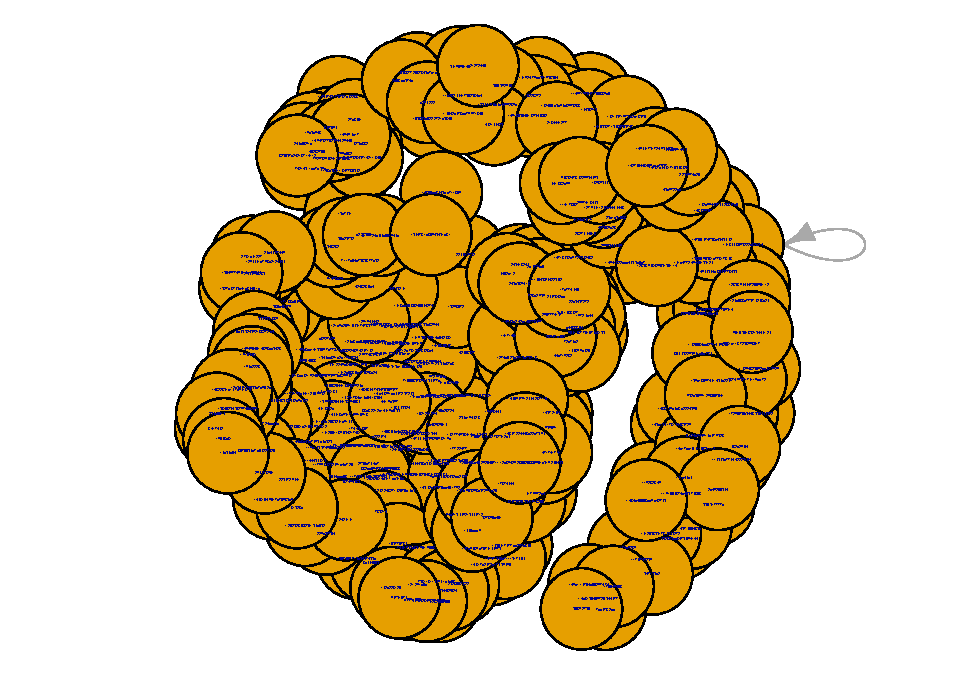
\includegraphics{SMI-Project-2022_files/figure-latex/unnamed-chunk-3-1.pdf}

\begin{Shaded}
\begin{Highlighting}[]
\CommentTok{\# Convert the directed graph into undirected graph}
\NormalTok{convertem }\OtherTok{\textless{}{-}} \FunctionTok{graph\_from\_data\_frame}\NormalTok{(datatw, }\AttributeTok{directed =} \ConstantTok{FALSE}\NormalTok{)}

\FunctionTok{par}\NormalTok{(}\AttributeTok{mar =} \FunctionTok{c}\NormalTok{(}\DecValTok{0}\NormalTok{, }\DecValTok{0}\NormalTok{, }\DecValTok{0}\NormalTok{, }\DecValTok{0}\NormalTok{))}
\FunctionTok{V}\NormalTok{(convertem)}\SpecialCharTok{$}\NormalTok{label.cex}\OtherTok{=}\FloatTok{0.1}
\FunctionTok{plot}\NormalTok{(convertem, }\AttributeTok{layout =}\NormalTok{ layout.fruchterman.reingold, }\AttributeTok{vertex.size =} \DecValTok{30}\NormalTok{)}
\end{Highlighting}
\end{Shaded}

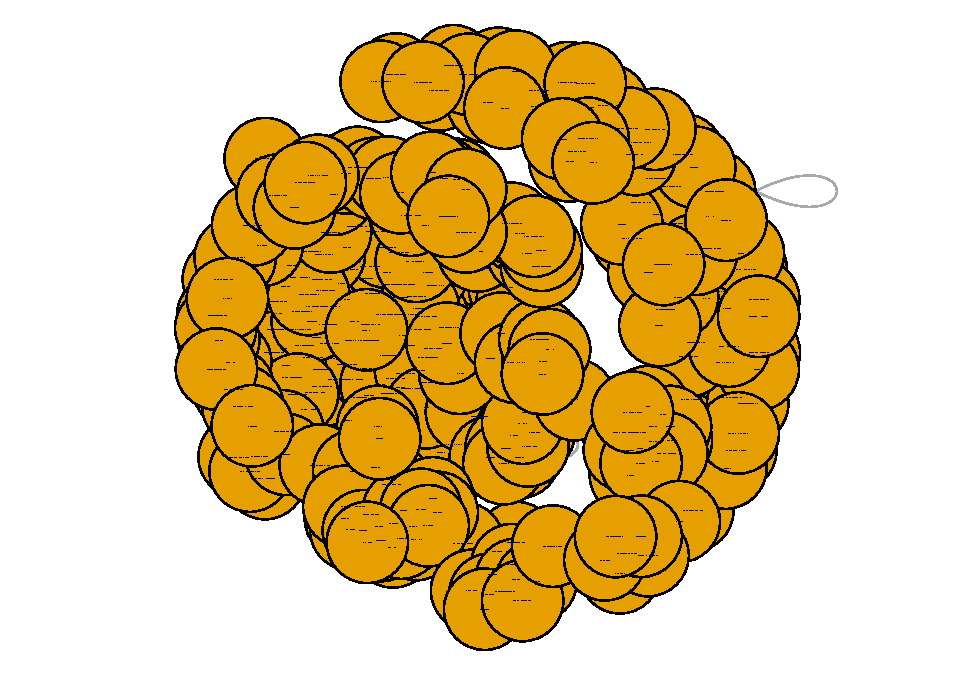
\includegraphics{SMI-Project-2022_files/figure-latex/unnamed-chunk-3-2.pdf}

\begin{Shaded}
\begin{Highlighting}[]
\CommentTok{\# Compute the number of components and size of each components}
\CommentTok{\# number of components}
\FunctionTok{count\_components}\NormalTok{(convertem)}
\end{Highlighting}
\end{Shaded}

\begin{verbatim}
## [1] 30
\end{verbatim}

\begin{Shaded}
\begin{Highlighting}[]
\CommentTok{\# size of each components}
\NormalTok{aa }\OtherTok{=} \FunctionTok{components}\NormalTok{(convertem)}
\NormalTok{aa}\SpecialCharTok{$}\NormalTok{csize}
\end{Highlighting}
\end{Shaded}

\begin{verbatim}
##  [1] 216   2   2   2   2   3   3   2   2   2   2   3   2   1   2   2   2   2   3
## [20]   2   2   2   2   4   2   2   2   6   2   2
\end{verbatim}

\begin{Shaded}
\begin{Highlighting}[]
\CommentTok{\# Plot the largest component of the graph}
\DocumentationTok{\#\# First split the components of the graph}
\NormalTok{deco }\OtherTok{=} \FunctionTok{decompose}\NormalTok{(convertem)}

\DocumentationTok{\#\# nodes number in each component}
\NormalTok{nc }\OtherTok{=} \FunctionTok{sapply}\NormalTok{(deco, }\ControlFlowTok{function}\NormalTok{(x) \{}\FunctionTok{length}\NormalTok{(}\FunctionTok{V}\NormalTok{(x))\})}

\DocumentationTok{\#\# index of largest component}
\NormalTok{lc }\OtherTok{=} \FunctionTok{which}\NormalTok{(nc }\SpecialCharTok{==} \FunctionTok{max}\NormalTok{(nc))}

\DocumentationTok{\#\# largest component\textquotesingle{}s edges}
\NormalTok{lce }\OtherTok{=}\NormalTok{ deco[[lc]]}

\DocumentationTok{\#\# largest component graph}
\NormalTok{lcgraph }\OtherTok{=} \FunctionTok{cluster\_edge\_betweenness}\NormalTok{(lce, }\AttributeTok{directed =} \ConstantTok{FALSE}\NormalTok{)}

\CommentTok{\# check all partition}
\FunctionTok{print}\NormalTok{(lcgraph}\SpecialCharTok{$}\NormalTok{membership)}
\end{Highlighting}
\end{Shaded}

\begin{verbatim}
##   [1]  1  1  2  3  4  5  1  6  7  1  1  1  1  1  1  8  1  9  7  1  1  2  1  1  1
##  [26]  5 10  1  1 11 10  1  2 12 13  2 14  1 15  4  4  7 16  1 17  1  1  1  3  1
##  [51]  1  1  1  1  4  1  1 18  7  1 17  1 19  2  1 14 20 20 21  1 22  7 21  1 20
##  [76] 23 20 24  1  1 25  1  1 26  2  7 27  1 28  1  1 29 30 23  1 31  1 32  7  2
## [101]  7  1 33 34  5  1  2  3  3  3  3  3  3  3  3  3  3  4 23  5  6  7  8  8  9
## [126]  1  5  5  5  5  5  5  5  5  5  5  5  5  5  5 10 11 11 10 10 10 10 10 12 13
## [151] 14 15  7 16 16 17 17 18 18 18 18 18 18 20 17 17 17 17 17 17 17 17 17 17 17
## [176] 17 17 17 17 17 17 17 17 19 14 20 20 20 20 20 21 22 20 20 20 20 24 25 25 25
## [201] 26 27 28 29 30 31 32 32  7 33 33 33 33 34  5  5
\end{verbatim}

\begin{Shaded}
\begin{Highlighting}[]
\CommentTok{\# check all the edges}
\FunctionTok{table}\NormalTok{(lcgraph}\SpecialCharTok{$}\NormalTok{membership) }
\end{Highlighting}
\end{Shaded}

\begin{verbatim}
## 
##  1  2  3  4  5  6  7  8  9 10 11 12 13 14 15 16 17 18 19 20 21 22 23 24 25 26 
## 47  8 12  5 20  2 11  3  2  8  3  2  2  4  2  3 23  7  2 14  3  2  3  2  4  2 
## 27 28 29 30 31 32 33 34 
##  2  2  2  2  2  3  5  2
\end{verbatim}

\begin{Shaded}
\begin{Highlighting}[]
\DocumentationTok{\#\# By checking all the edges, the highest number is 1, so we use 1 as the largest component}
\NormalTok{lcno }\OtherTok{=} \DecValTok{1}
\NormalTok{indexlc }\OtherTok{=} \FunctionTok{which}\NormalTok{(lcgraph}\SpecialCharTok{$}\NormalTok{membership }\SpecialCharTok{==}\NormalTok{ lcno)}

\DocumentationTok{\#\# Taking the nodes from largest component to be plotted}
\NormalTok{lcgraphed }\OtherTok{=} \FunctionTok{subgraph}\NormalTok{(deco[[lc]], indexlc)}
\end{Highlighting}
\end{Shaded}

\begin{verbatim}
## Warning in subgraph(deco[[lc]], indexlc): At
## structural_properties.c:2051 :igraph_subgraph is deprecated from igraph 0.6, use
## igraph_induced_subgraph instead
\end{verbatim}

\begin{Shaded}
\begin{Highlighting}[]
\FunctionTok{plot}\NormalTok{(lcgraphed, }\AttributeTok{vertex.size=}\DecValTok{5}\NormalTok{)}
\end{Highlighting}
\end{Shaded}

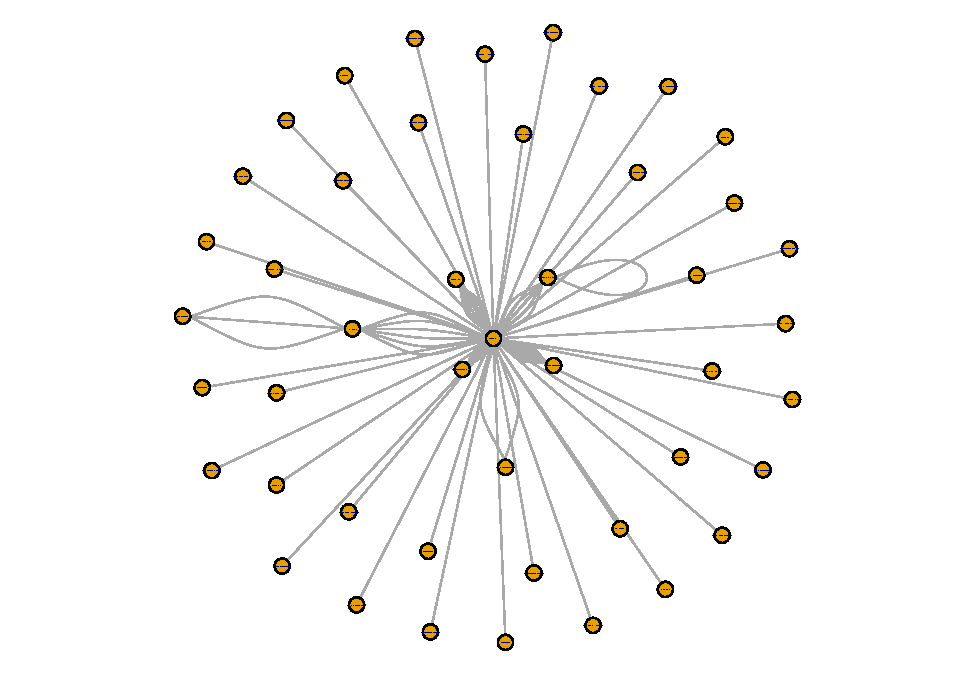
\includegraphics{SMI-Project-2022_files/figure-latex/unnamed-chunk-3-3.pdf}

\begin{Shaded}
\begin{Highlighting}[]
\DocumentationTok{\#\# Graph partition by hierarchical relationship}
\FunctionTok{plot}\NormalTok{(}\FunctionTok{as.dendrogram}\NormalTok{(lcgraph)) }
\end{Highlighting}
\end{Shaded}

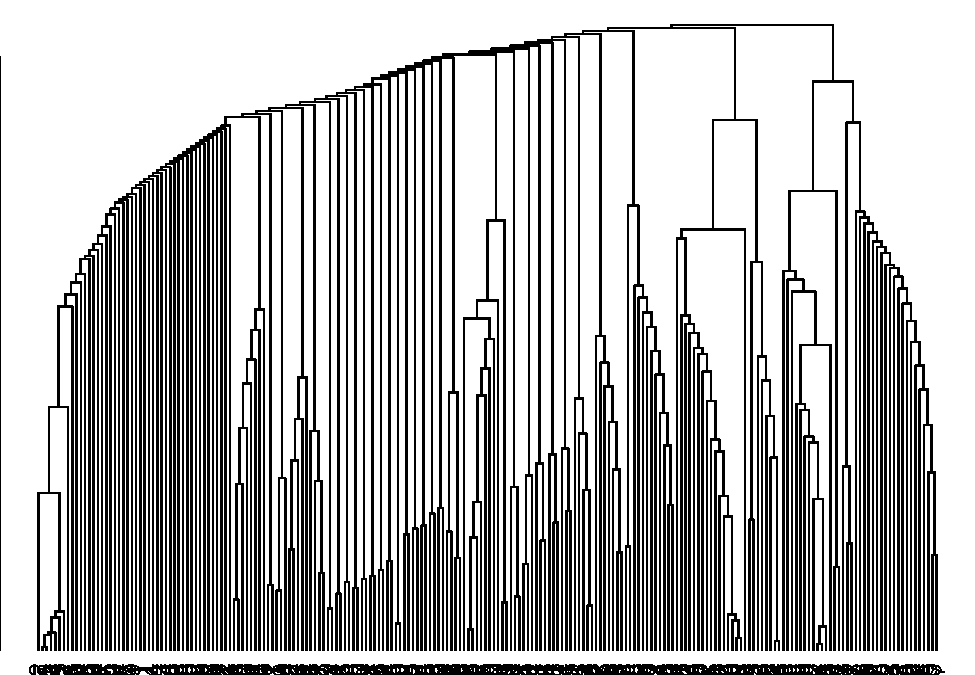
\includegraphics{SMI-Project-2022_files/figure-latex/unnamed-chunk-3-4.pdf}

\begin{enumerate}
\def\labelenumi{\arabic{enumi}.}
\setcounter{enumi}{2}
\tightlist
\item
  Graph Statistics
\end{enumerate}

\begin{Shaded}
\begin{Highlighting}[]
\CommentTok{\# graph diameter}
\FunctionTok{diameter}\NormalTok{(lcgraphed)}
\end{Highlighting}
\end{Shaded}

\begin{verbatim}
## [1] 3
\end{verbatim}

\begin{Shaded}
\begin{Highlighting}[]
\CommentTok{\# graph density}
\FunctionTok{graph.density}\NormalTok{(lcgraphed)}
\end{Highlighting}
\end{Shaded}

\begin{verbatim}
## [1] 0.08233117
\end{verbatim}

\begin{Shaded}
\begin{Highlighting}[]
\CommentTok{\# plotting the degree distribution of the graph}
\FunctionTok{degree}\NormalTok{(lcgraphed)}
\end{Highlighting}
\end{Shaded}

\begin{verbatim}
## 1334440824608706562 1464529166557237253  710008378945355776 1523178461560418304 
##                   1                  18                   1                   2 
##  886822126145196033           158553324 1176088924894257152 1436568756331839492 
##                   8                   7                   1                   1 
##          3165824401            97297046 1331224968407891970 1316630499738021889 
##                   1                   1                   1                   1 
##           363762075 1519396939736829952 1483070768980316160 1475554039890952196 
##                   9                   1                   1                   1 
## 1455186931759910918 1484854743470309377            45152326  901313610806251520 
##                   1                   7                   1                   1 
## 1450820441803829256  837126781282852864          2977485983  908701589170352128 
##                   1                   1                   1                   1 
##            16222574 1480481160820109319           156198185            40628724 
##                   1                   1                   1                   1 
## 1488327858518999044           174451807 1522034108788281344 1445628693376684040 
##                   1                   1                   1                   1 
## 1408056463331758081 1512608806575898624 1512001189034217481 1521059182451036161 
##                   1                   1                   1                   1 
## 1531579300947759105 1256866059098955777 1345668916261965824 1241807750432206848 
##                   1                   1                   1                   1 
##  927032191233568768 1399302045413294085          2648989015 1511636208325169155 
##                   1                   1                   1                   1 
##          1021241294            44196397          1291945442 
##                   1                  85                   3
\end{verbatim}

\begin{Shaded}
\begin{Highlighting}[]
\FunctionTok{max}\NormalTok{(}\FunctionTok{degree}\NormalTok{(lcgraphed))}
\end{Highlighting}
\end{Shaded}

\begin{verbatim}
## [1] 85
\end{verbatim}

\begin{Shaded}
\begin{Highlighting}[]
\NormalTok{dd }\OtherTok{=} \FunctionTok{degree.distribution}\NormalTok{(lcgraphed)}
\FunctionTok{hist}\NormalTok{(dd)}
\end{Highlighting}
\end{Shaded}

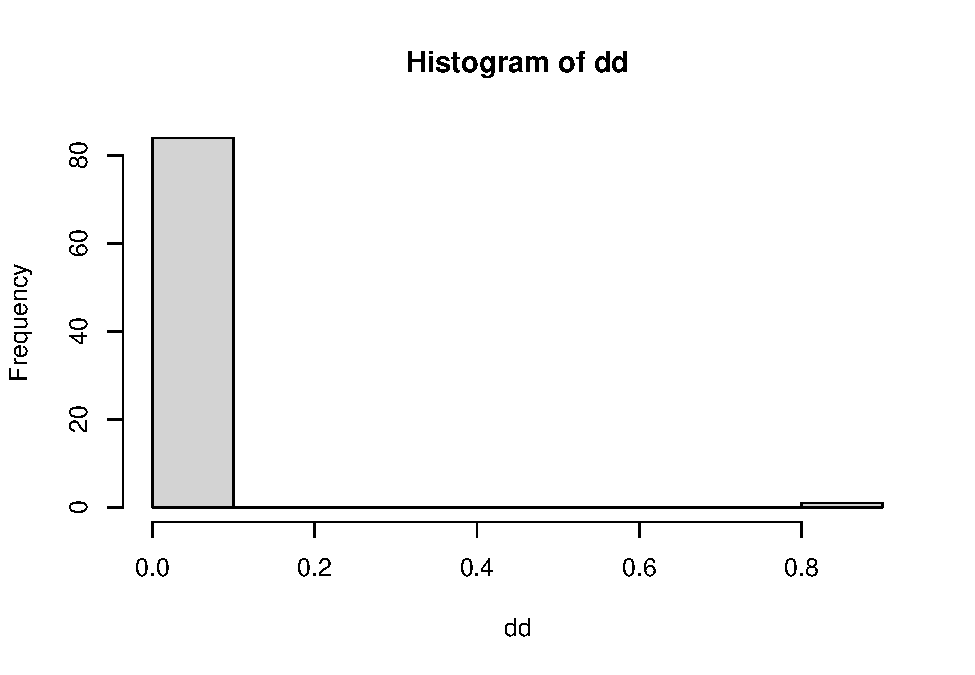
\includegraphics{SMI-Project-2022_files/figure-latex/unnamed-chunk-4-1.pdf}

\begin{Shaded}
\begin{Highlighting}[]
\CommentTok{\# estimating the Power Law coefficient(c) from the degree distribution}
\NormalTok{pl }\OtherTok{=} \FunctionTok{fit\_power\_law}\NormalTok{(dd, }\AttributeTok{xmin =} \FloatTok{0.000000000000000001}\NormalTok{)}
\FunctionTok{print}\NormalTok{(pl)}
\end{Highlighting}
\end{Shaded}

\begin{verbatim}
## $continuous
## [1] TRUE
## 
## $alpha
## [1] 1.026219
## 
## $xmin
## [1] 1e-18
## 
## $logLik
## [1] -10.68584
## 
## $KS.stat
## [1] 0.6268302
## 
## $KS.p
## [1] 0.003721941
\end{verbatim}

\begin{Shaded}
\begin{Highlighting}[]
\FunctionTok{print}\NormalTok{(pl)}\SpecialCharTok{$}\NormalTok{alpha}
\end{Highlighting}
\end{Shaded}

\begin{verbatim}
## $continuous
## [1] TRUE
## 
## $alpha
## [1] 1.026219
## 
## $xmin
## [1] 1e-18
## 
## $logLik
## [1] -10.68584
## 
## $KS.stat
## [1] 0.6268302
## 
## $KS.p
## [1] 0.003721941
\end{verbatim}

\begin{verbatim}
## [1] 1.026219
\end{verbatim}

\begin{verbatim}
4. Information Flow


```r
# neighourhood overlap between each pair of connected nodes in the twitter graph 
# changing the name of the vertex to easier analysis process
bb = set.vertex.attribute(lcgraphed, "name", value = paste("A",1:146, sep = ""))
\end{verbatim}

\begin{verbatim}
## Warning in vattrs[[name]][index] <- value: number of items to replace is not a
## multiple of replacement length
\end{verbatim}

\begin{Shaded}
\begin{Highlighting}[]
\NormalTok{en }\OtherTok{=} \FunctionTok{ends}\NormalTok{(bb, }\FunctionTok{E}\NormalTok{(bb), }\AttributeTok{names =} \ConstantTok{FALSE}\NormalTok{)}

\NormalTok{ne.over }\OtherTok{=} \ControlFlowTok{function}\NormalTok{(no1, no2, graphed) \{}
\NormalTok{  i }\OtherTok{=} \FunctionTok{intersection}\NormalTok{(}\FunctionTok{neighbors}\NormalTok{(graphed, no1), }\FunctionTok{neighbors}\NormalTok{(graphed, no2))}
\NormalTok{  u }\OtherTok{=} \FunctionTok{union}\NormalTok{(}\FunctionTok{neighbors}\NormalTok{(graphed, no1), }\FunctionTok{neighbors}\NormalTok{(graphed, no2))}
\NormalTok{  a }\OtherTok{=} \FunctionTok{length}\NormalTok{(i)}\SpecialCharTok{/}\NormalTok{ (}\FunctionTok{length}\NormalTok{(u)) }
  \FunctionTok{return}\NormalTok{(a)}
\NormalTok{\}}

\NormalTok{nodes }\OtherTok{=} \FunctionTok{list}\NormalTok{()}

\ControlFlowTok{for}\NormalTok{ (i }\ControlFlowTok{in} \FunctionTok{seq}\NormalTok{(}\FunctionTok{nrow}\NormalTok{(en)))\{}
\NormalTok{  node1 }\OtherTok{=}\NormalTok{ en[i, }\DecValTok{1}\NormalTok{]}
\NormalTok{  node2 }\OtherTok{=}\NormalTok{ en[i, }\DecValTok{2}\NormalTok{]}
\NormalTok{  nover }\OtherTok{=} \FunctionTok{ne.over}\NormalTok{(}\AttributeTok{no1 =}\NormalTok{ node1, }\AttributeTok{no2 =}\NormalTok{ node2, }\AttributeTok{graphed =}\NormalTok{ bb)}
\NormalTok{  nodes[i] }\OtherTok{=}\NormalTok{ nover}
\NormalTok{\}}


\CommentTok{\# identify the pair with the greatest and least neighborhood overlap}
\NormalTok{d }\OtherTok{=} \FunctionTok{c}\NormalTok{()}

\ControlFlowTok{for}\NormalTok{ (i }\ControlFlowTok{in} \DecValTok{1}\SpecialCharTok{:}\FunctionTok{length}\NormalTok{(nodes))\{}
\NormalTok{  d[i] }\OtherTok{=}\NormalTok{ nodes[[i]][}\DecValTok{1}\NormalTok{]}
\NormalTok{\}}

\NormalTok{l }\OtherTok{=}\NormalTok{ d[}\FunctionTok{order}\NormalTok{(d,}\AttributeTok{decreasing=}\ConstantTok{TRUE}\NormalTok{)]}
\CommentTok{\#l}
\end{Highlighting}
\end{Shaded}


\end{document}
